\documentclass{article}
\usepackage{graphicx}
\begin{document}

\section{Look Ahead}
\subsection{Theory of Operation}
The look ahead node is responsible for obstacle detection. The node subscribes
to lidar data to and uses trigonometric functions create a configuration space
that resembles a bounded box. The configuration space is determined by creat-
ing a box of lidar pings slightly larger than the perimeter of the robot (1m by
0.5m). The C-Space is directly in front of the robot. Below is a list of Constants
used in the look ahead source file:\\
const uint cPings = 181; The data from the laser comes from the topic sensor$\textunderscore$msgs$\backslash$LaserScan
and is passed into an array large enough to hold 181 values (one for each ping)\\
const double cBoxHeight = 1.0; This value corresponds to the height of the\\
c-space bounded box
const double cBoxWidth = 0.5; This value corresponds to the width of the
c-space bounded box
The node constantly publishes to a custom message type called “obstacles.”
If an obstacle is found within the configuration space then the look ahead node
publishes true (an obstacle exists) and the obstacle’s distance along the current
path, otherwise the node publishes false for the obstacles existence and 0 for its
distance. Obstacle detection is mathematically derived. If a lidar ping returns
and it is less than the height or width of the c-space divided by cos$\theta$ where $\theta$ is
in radians then an obstacle exists.\\\\

$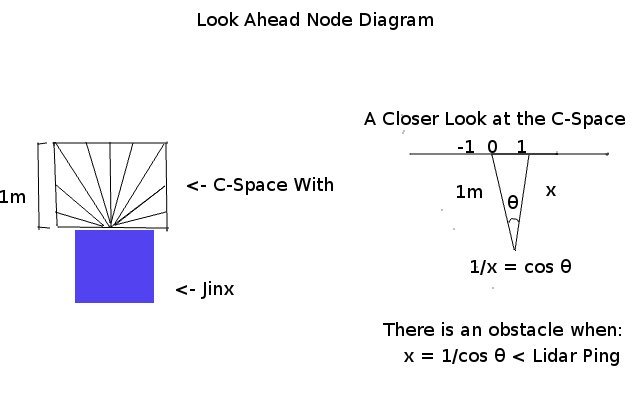
\includegraphics[scale = 0.5]{look_ahead.jpg}$ \\
Figure 1 - Represented by lines 56 - 77

Figure 1 is reproduced in our code through this example:\\\\
\indent if(curLaserData[i] $<$ cBoxWidth/cos((180.0-(double)i)*M PI/180.0))\\
\indent \indent$\{$\\
\indent \indent \indent if(curLaserData[i] $<$ closestObs)\\
\indent \indent \indent$\{$\\
\indent \indent closestObs = curLaserData[i];\\
\indent \indent \indent$\}$\\
\indent \indent$\}$\\
The above code snippet means that if the lidar ping is less than the width of the bounded box divided by cos$\theta$ an obstacle exists and its distance is the distance the lidar ping returns.\\

After the algorithim was properly developed one inital problem with the look ahead code was the lidars 80m
range. In order to make sure that lidar data was not misinterpreted beyond
the bounds of the box we created a value of closestObs and set it to 90(m).
Since the lidars range is 80 there shoudld definetley not be any object detected
beyond the length of closestObs.

\subsection{Observations}
Lidar detection obstacle detection is not good while turning. There seems to be
a blind spot right next to the lidar scanner.

\subsection{Future Plans}
Presently our c-space configuration algorithim will not suffice for arced paths. We plan on doing some modifications to the look ahead source code to ensure the robots ability to detect obstacles at any given instance. The node will aslo need to receive segment status messages to determine if there is an obstacle path on the type of path the robot is considering moving along.

\end{document}




